\documentclass[11pt]{article}

\usepackage{fancyhdr}
\usepackage{graphicx}
\usepackage{geometry}
\usepackage{lastpage}
\usepackage{titling}
\usepackage{sectsty}
\usepackage{setspace}
\usepackage{changepage}
\usepackage[shortlabels]{enumitem}
\usepackage{subcaption}
\usepackage{helvet}
\usepackage{tabularx}

\usepackage{siunitx}
\usepackage{nicefrac}
\usepackage{amsmath}
\usepackage{gensymb}
\usepackage{amssymb}
\usepackage{float}
\setcounter{MaxMatrixCols}{11}
\usepackage{indentfirst}

\usepackage{listings}
\usepackage{matlab-prettifier}
% \usepackage{color}
% \definecolor{dkgreen}{rgb}{0,0.6,0}
% \definecolor{gray}{rgb}{0.5,0.5,0.5}
% \definecolor{mauve}{rgb}{0.58,0,0.82}

\lstset
{
  frame=tb,
  style=Matlab-editor,
  % language=MATLAB, %Matlab-editor,
  aboveskip=3mm,
  belowskip=3mm,
  showstringspaces=false,
  columns=flexible,
  basicstyle={\small\ttfamily},
  numbers=none,
  % numberstyle=\tiny\color{gray},
  % keywordstyle=\color{blue},
  % commentstyle=\color{dkgreen},
  % stringstyle=\color{mauve},
  breaklines=true,
  breakatwhitespace=true,
  tabsize=3
}

\geometry
{
  letterpaper, 
  total={175.9mm,229.4mm}, 
  top=25mm, 
  left=20mm, 
  headheight=26pt,
  voffset=12pt,
  footskip=15pt
}
\author{Daniel Sturdivant}
\title{Lab 3}
\date{March 2023}
\graphicspath{ {./media/} }

\pagestyle{fancy}
\fancyhead[R]{March 17, 2023}
\fancyhead[L]{Sturdivant, Daniel \\ Weir, Andrew}
\fancyhead[C]{MECH 6970 GPS}
\fancyfoot[C]{Page \thepage\ of \pageref{LastPage}}

\makeatletter
\def\@maketitle
{
  \null
  \begin{center}
    {\huge \@title \\}
  \end{center}
  \vskip 5mm
}
\makeatother

\sectionfont{\fontsize{16}{16}}
\subsectionfont{\fontsize{13}{13}\normalfont}
\renewcommand{\thesubsection}{\arabic{section}-\arabic{subsection}}
\renewcommand{\familydefault}{\sfdefault}
\newcommand{\solution}{\textbf{Solution: \\}}


%% ====================================================================== %%
\begin{document}

\maketitle
\thispagestyle{fancy}
\setstretch{1.25}
% \setlength{\parskip}{0em}
% \setlength{\abovedisplayskip}{-8pt}
% \setlength{\belowdisplayskip}{12pt}
\setlength{\parindent}{0pt}

\begin{enumerate}[label=\textbf{\arabic*.}]
  \itemsep 24pt
  \item \textbf{Improved GPS Positioning} \\
Whether it is noise or an atmospheric disturbances, GPS positioning inherently involves some error. To combat this error, different methods
can be used to correct the raw measurements. In this section, different methods are used to correct the positioning of a static Novatel receiver. 
This receiver was located in the Auburn MRI, and data was taken on March 16, 2023 at a 1 Hz sample rate. To start, an initial GPS position 
solution for the static data set was determined using a Gauss-Newton least squares approach. The least squares equation is given as:
    \begin{equation}
          x =(G^T\ G)^{-1}\ G^T\ y
    \end{equation}
  where \textit{x} is the state vector including the position and clock bias differentials, \textit{G} is the geometry matrix, and \textit{y} is 
  the difference between the pseudorange and range. To determine the static position solution, only the 8 satellites that had both L1 and L2 
  pseudoranges for the entire data set were used. This was done so that the amount of satellites used in each solution method would remain 
  constant. Any improvements in positioning would be a consequence of removing error not removing or adding satellites. Figure 1 gives the position solution for the static data set. 
    \begin{figure}[H]
        \centering
        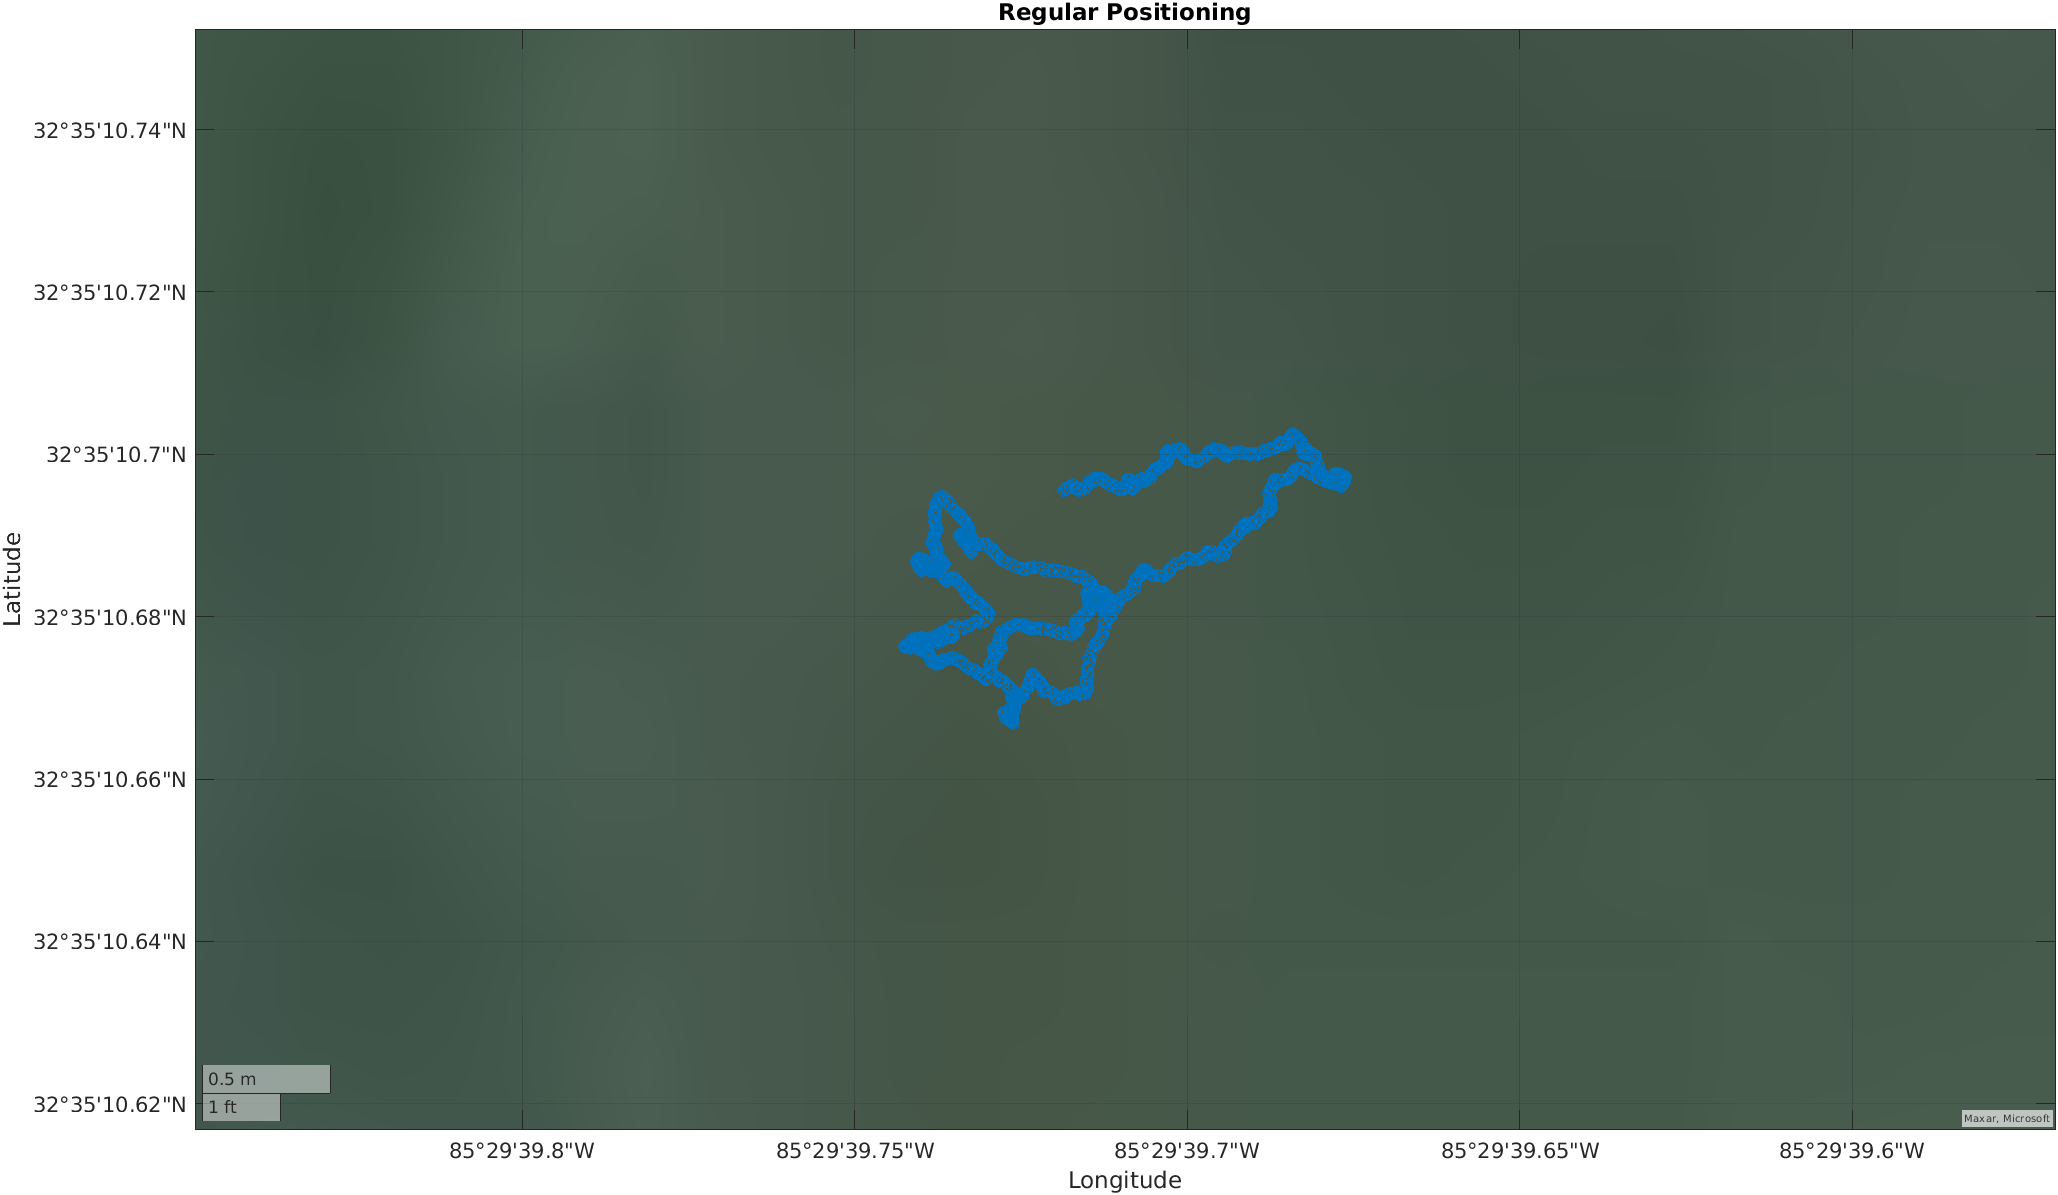
\includegraphics[width=0.7\textwidth]{p1_a.png}
        \caption{Static GPS Position Solution.}
    \end{figure}
  After determining the static GPS position solution carrier phase smoothing was performed to mitigate the measurement noise. Carrier phase smoothing utilizes the relative distance on a less noisy carrier phase measurement to average the pseudorange over a window. The equation for carrier phase smoothing is given as:
    \begin{equation}
        \overline\rho\ (t_i\ )=\dfrac{1}{M}\ \rho(t_i\ )+\dfrac{M-1}{M}(\overline\rho\ (t_i-1)+\phi(t_i\ )-\phi(t_i-1))
    \end{equation}
  where \textit{$\overline\rho$} is the averaged pseudorange, \textit{M} is the averaging window, \textit{$t_i$} is the current time step, and \textit{$\phi$} is the carrier phase. Increasing the averaging window allows for more smoothing but could introduce a bias. Therefore window sizes of 2, 8, and 15 minutes were used as averaging windows and compared against each other. To generate a position solution the same Gauss-Newton least squares method is used but with the averaged pseudorange. Figure 2 shows the carrier phase smoothed GPS position solutions for each averaging window along with the regular GPS position solution. 
    \begin{figure}[H]
        \centering
        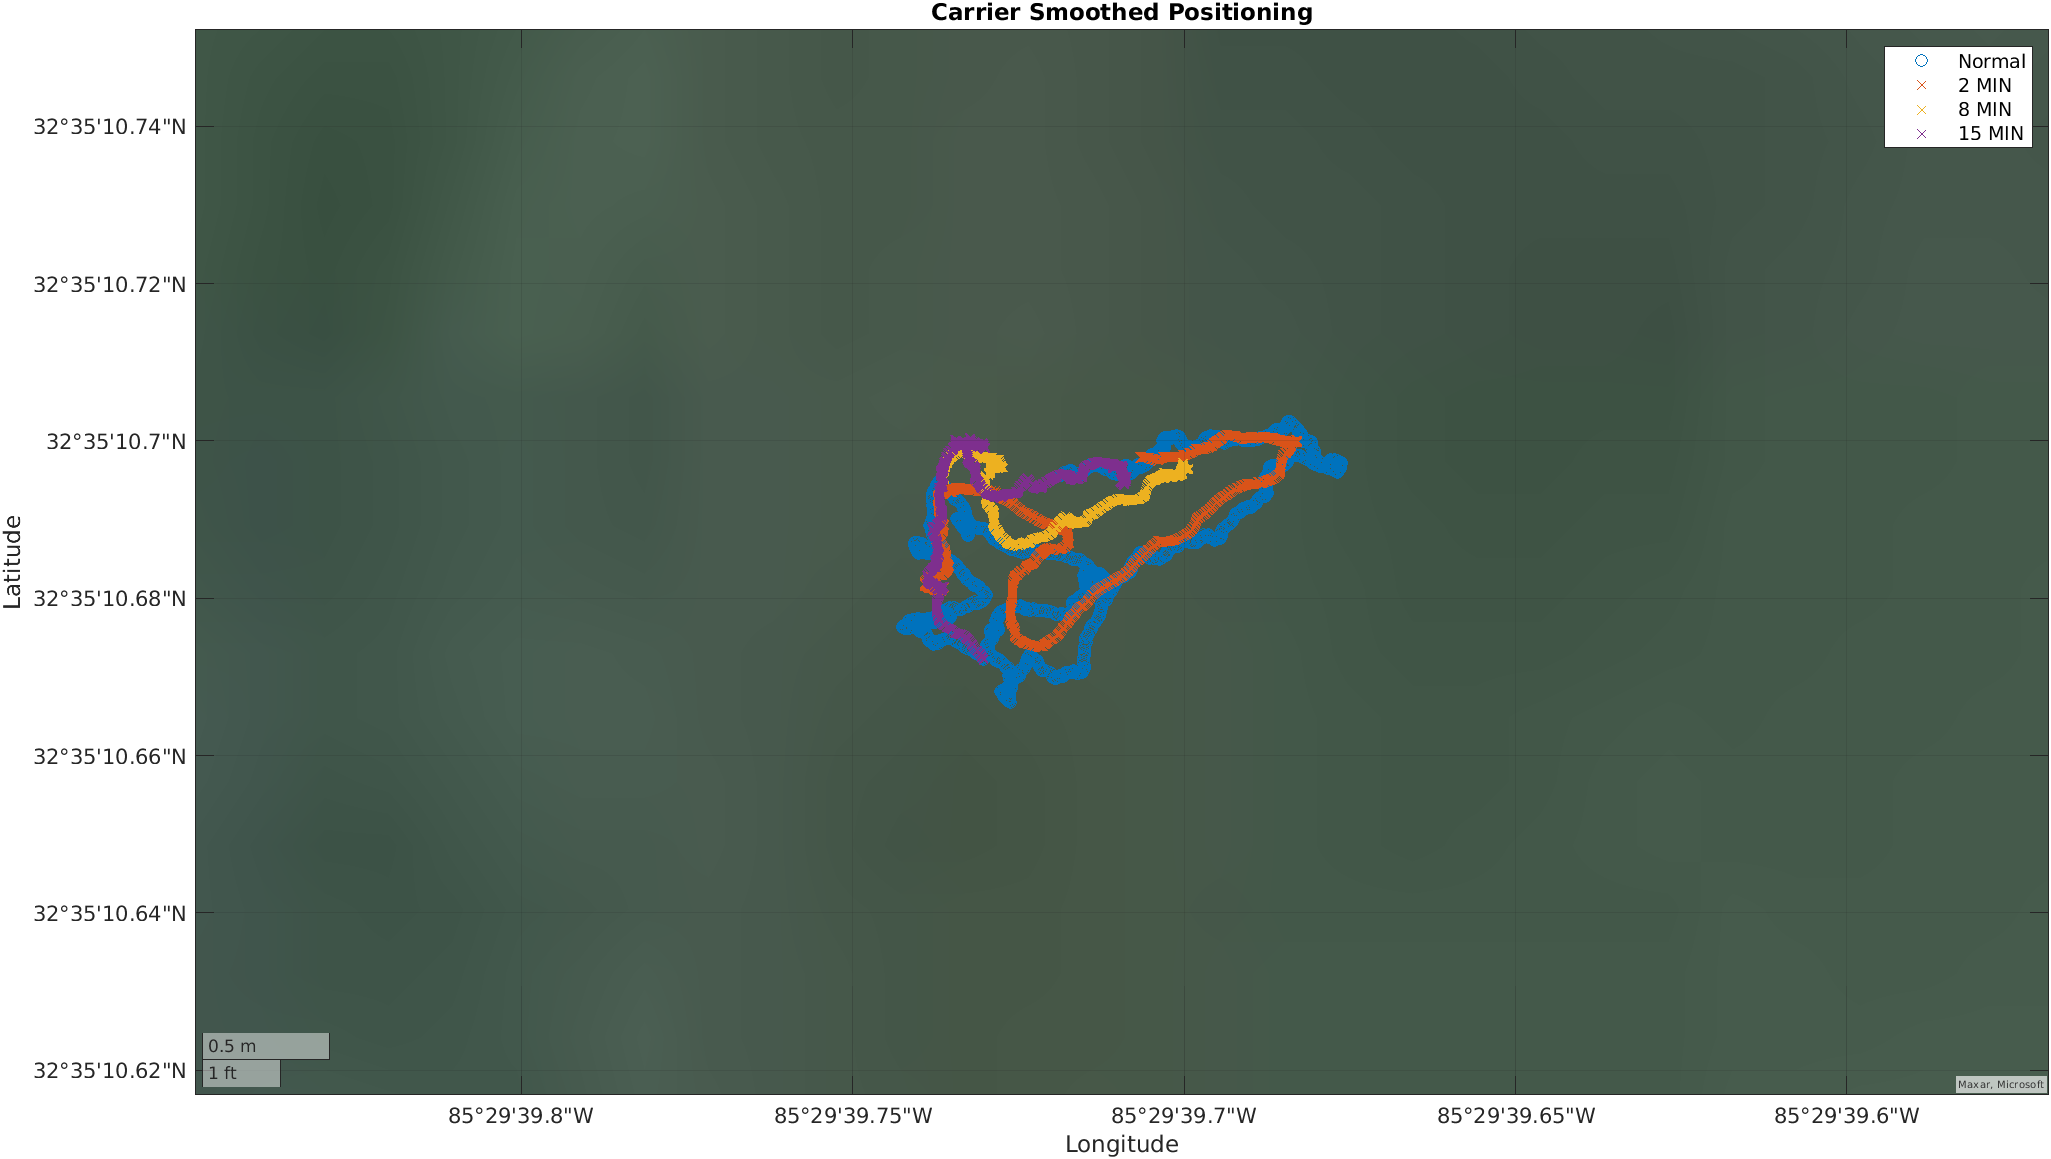
\includegraphics[width=0.7\textwidth]{p1_b.png}
        \caption{Carrier Smoothing GPS Position Solution.}
    \end{figure}
From figure 2, it can be seen that increasing the averaging window tightens the position solution. A smoother pseudorange measurement limits the amount of variance on the position solution. For the static scenario, an inclusion of a new bias is not seen for any of the averaging windows. Therefore, the higher 15 minute averaging window would be the preferred averaging window. The next method used to reduce the static position error was implementing an ephemeris ionosphere error model. This method estimates the atmospheric error due to the ionosphere and removes it from the pseudorange measurements. The equation for calculating the ionosphere correction term, taken from the GPS Interface Control Document is given as:
    \begin{equation}
    T_{iono}=\begin{cases}
    F*[5\times10^{-9}+AMP(1-\dfrac{x^2}{2}+\dfrac{x^4}{24}), & |x|<1.57]\\
    F*(5\times10^{-9}) & |x|\geq 1.57
    \end{cases}
    \end{equation}
where \textit{$T_{iono}$} is the ionosphere correction term, \textit{F} is the obliquity factor, and \textit{x} is the phase. This ionosphere is subtracted from the pseudorange, and a new position solution is calculated. Figure 3 shows the GPS position solution using the ephemeris ionosphere model correction as well as the original GPS position solution.
   \begin{figure}[H]
        \centering
        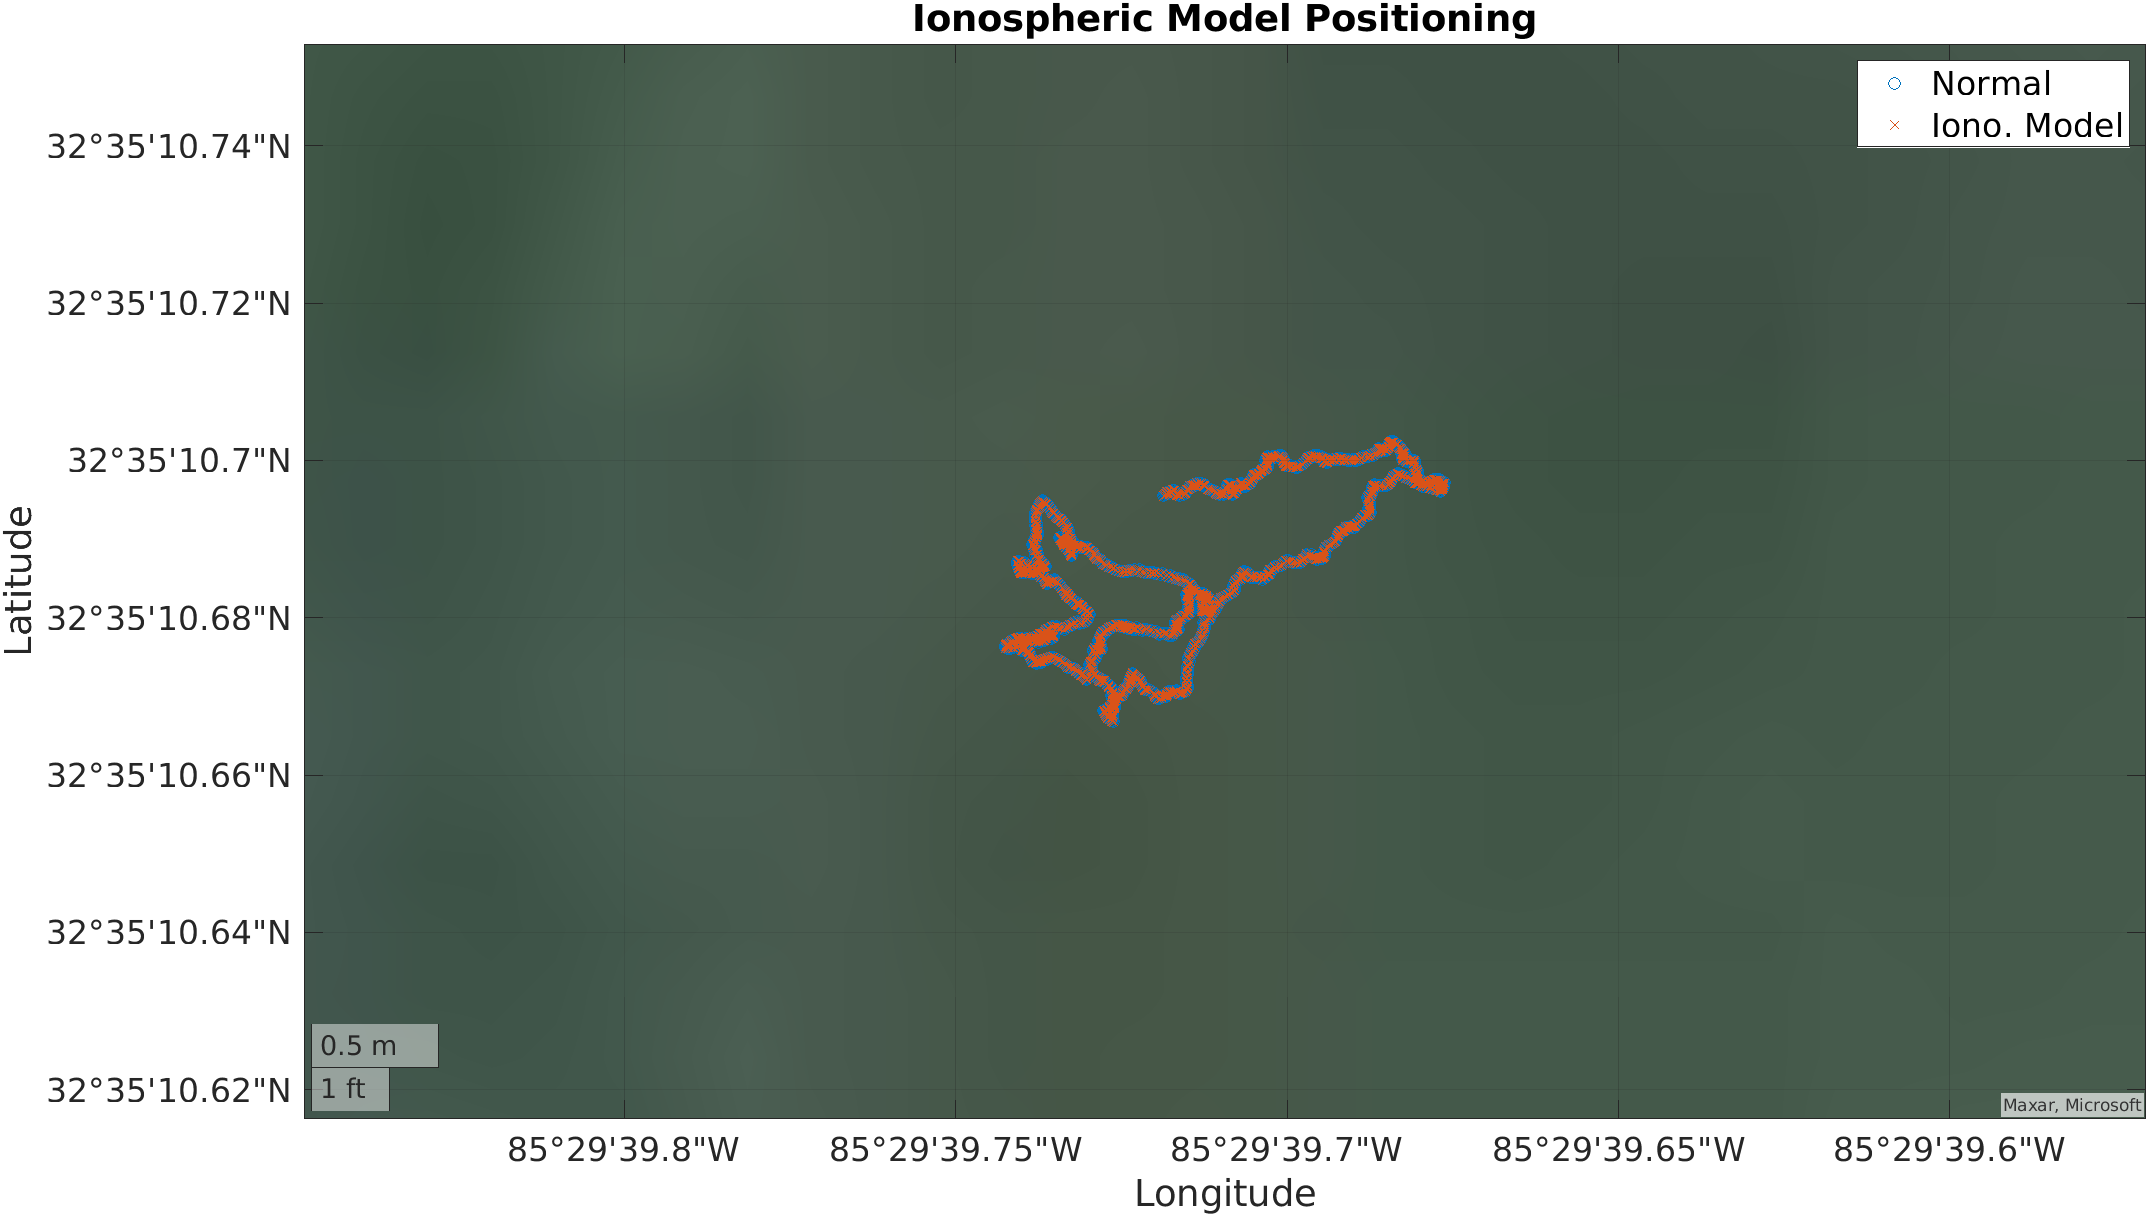
\includegraphics[width=0.7\textwidth]{p1_c.png}
        \caption{Ephemeris Model Correction GPS Position Solution.}
    \end{figure}
The ephemeris ionosphere model correction did not have much of an effect on the position solution. This id due to low amounts of ionosphere error being present in the data set to begin with. Another method of mitigating the ionosphere error is to use dual frequency to produce ionosphere free measurements. The error due to the ionosphere differs based on the signal frequency. By comparing pseudorange measurements at different frequencies, the error due to the ionosphere can be ascertained. The equation for an ionosphere free pseudorange is given by:
    \begin{equation}
        \rho_{IF}=\dfrac{f_{L1}^2}{(f_{L1}^2-f_{L2}^2)}\rho_{L1}-\dfrac{f_{L2}^2}{(f_{L1}^2-f_{L2}^2)}\rho_{L2}
    \end{equation}
where \textit{$\rho_{IF}$} is the ionosphere free pseudorange, \textit{$f_{L1}$} is the L1 frequency, and \textit{$f_{L2}$} is the L2 frequency. This ionospehere free pseudorange is used to create a new position solution. Figure 4 shows the GPS position solution using the dual frequency ionosphere free measurements and the original position solution. 
     \begin{figure}[H]
        \centering
        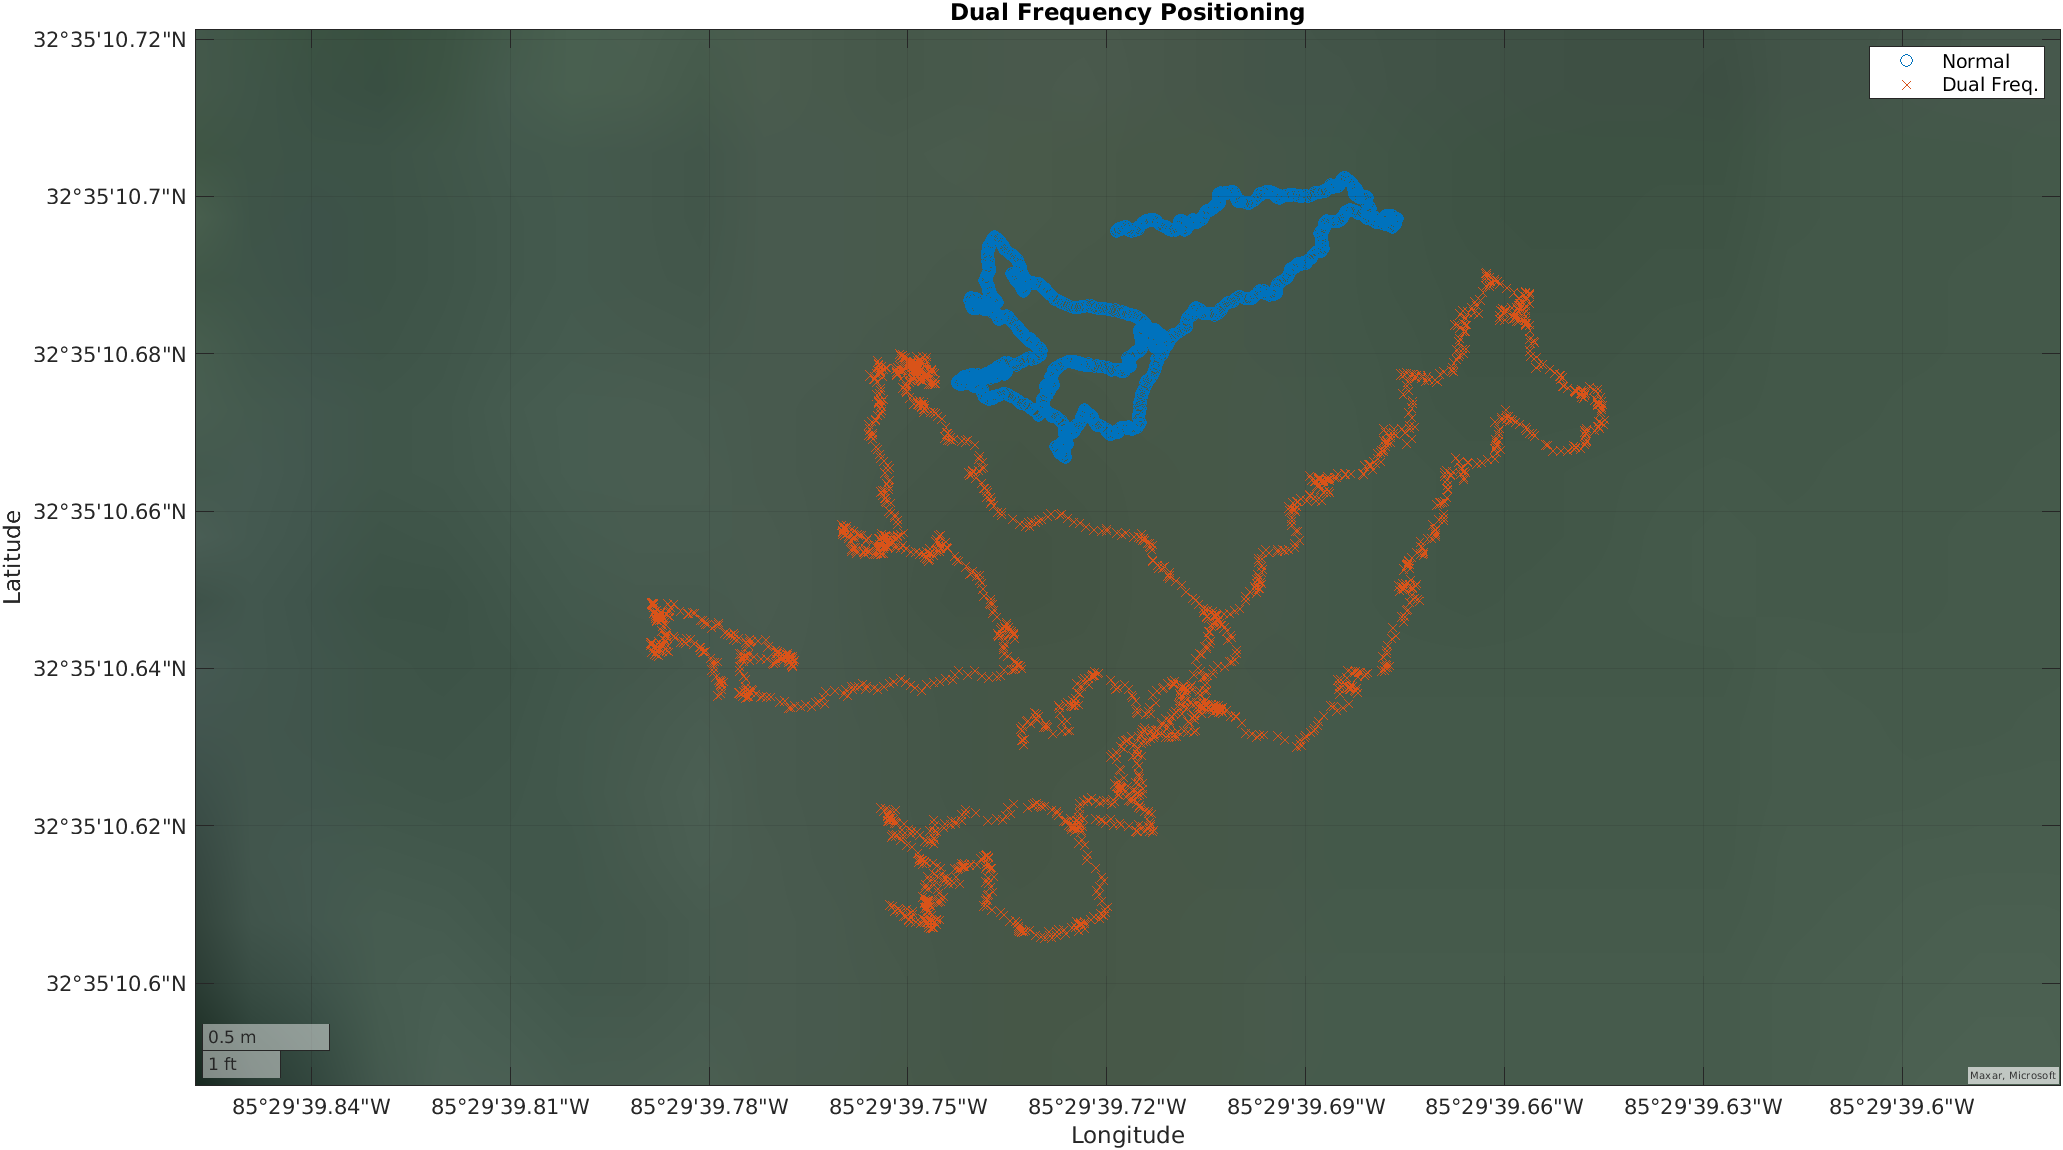
\includegraphics[width=0.7\textwidth]{p1_d.png}
        \caption{Dual Frequency Ionosphere Free GPS Position Solution.}
    \end{figure}
From figure 4 it can be seen that the position solution with the ionosphere free measurements moves to a new general location. This is due to the removal of the ionosphere error. However, it is also shown that the new position solution is much more  when compared to the original position solution. Since the error is added from both the L1 and L2 signals, the position solution will show more variance. Each of the static positions solutions are plotted against each other in figure 5. Additionally, table 1 gives the mean position in latitude and longitude as well as the standard deviation of the ECEF positions.
    \begin{figure}[H]
        \centering
        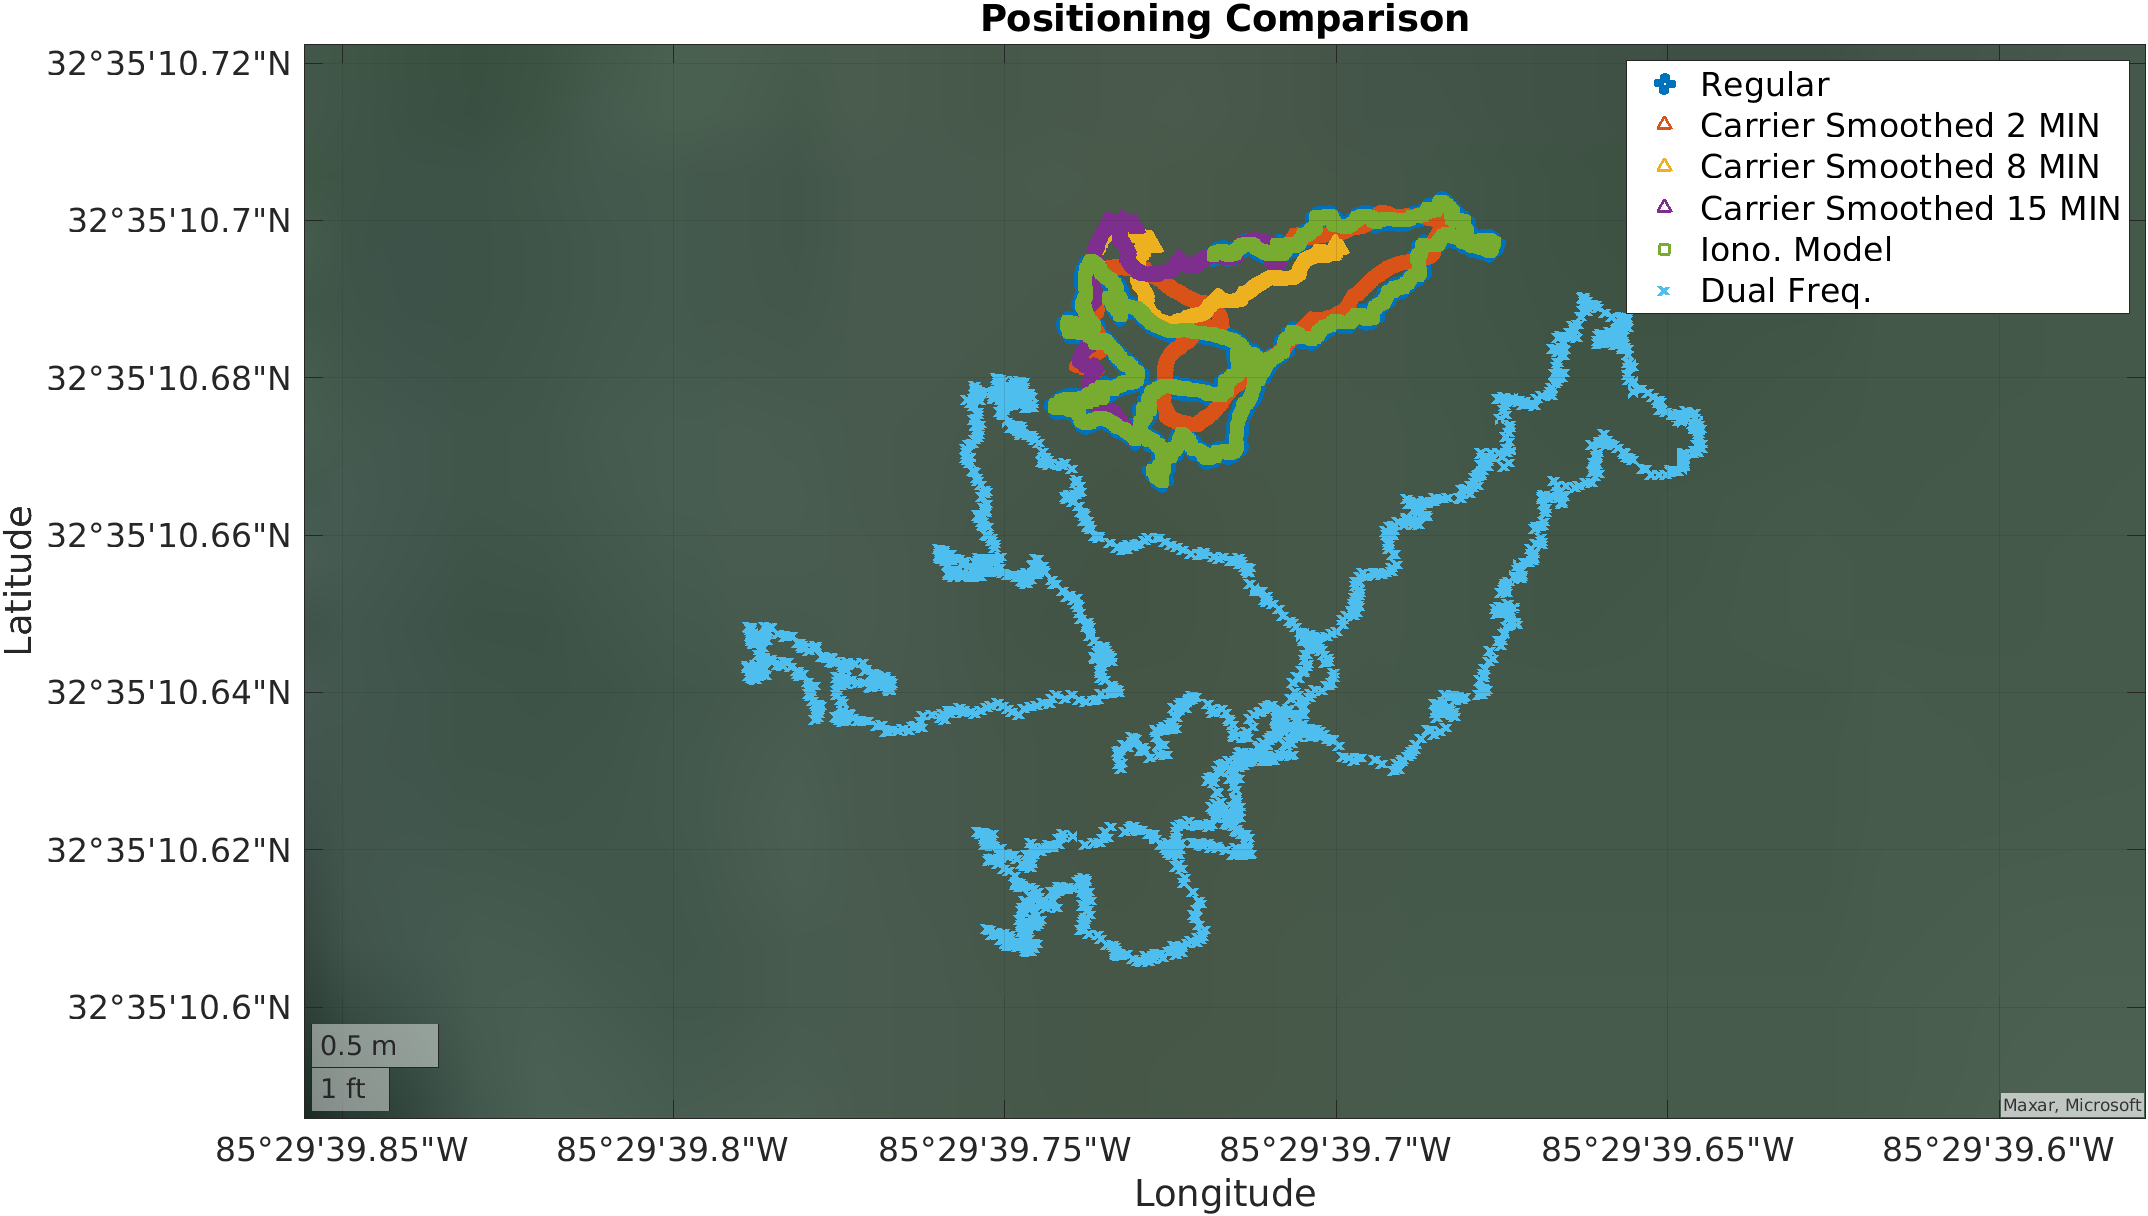
\includegraphics[width=0.7\textwidth]{p1_f.png}
        \caption{Dual Frequency Ionosphere Free GPS Position Solution.}
    \end{figure}
    \break
       \begin{center}
       \captionof{table}{Statistics for Static Position Solutions}
            \begin{tabularx}{0.85\textwidth} { 
            | >{\centering\arraybackslash}X 
              | >{\centering\arraybackslash}X 
              | >{\centering\arraybackslash}X 
              | >{\centering\arraybackslash}X 
              | >{\centering\arraybackslash}X 
              | >{\centering\arraybackslash}X  
              | >{\centering\arraybackslash}X | }
              \hline            & \textbf{Mean Latitude (\degree)} & \textbf{Mean Longitude (\degree)} & \textbf{X Std (m)} & \textbf{Y Std (m)} & \textbf{Z Std (m)}  \\
              \hline \textbf{Regular} & 32.586302    & -85.494366      & 0.533176    & 0.651778  & 0.734229 \\
              \hline \textbf{Carrier Smooth (2min)} & 32.586302 & -85.494366    & 0.509196  & 0.553659   & 0.623999  \\
              \hline \textbf{Carrier Smooth (8min)} & 32.586303 & -85.494368  & 0.361699 & 0.190694  & 0.318260 \\
              \hline \textbf{Carrier Smooth (15min)} & 32.586304 & -85.494369  & 0.245047 & 0.252832 & 0.245292   \\
              \hline \textbf{Ephemeris Ionosphere Model} & 32.586302 & -85.494366 & 0.533176 & 0.651778  & 0.734229  \\
              \hline \textbf{Dual Frequency Ionosphere Free} & 32.586291 & -85.494367  & 0.945983 & 1.391230 & 1.252064 \\
              \hline
    \end{tabularx}
  \end{center}

  
  From figure 5 and table 1 it can be seen that each of the position solutions are located in a similar location. The only position solution that is located farther than 1 meter away from the others is the dual frequency position solution. The dual frequency positioning is on average about 8 meters away from the original positioning solution. This is due to the removal of the ionosphere error, which removes a bias in the measurements. However, this position solution also has the highest standard deviation. This is due to the noise on the measurements being increased since two different pseudoranges are used. The positioning solution with the lowest standard deviation is the carrier smoothed positioning solution with a 15 minute averaging window. The noise on the measurements was mitigated using the more precise carrier phase measurements, leading to less position variance. The ionosphere model position solution has the least amount of impact on the original solution. The mean and standard deviation for each position solution are about the same. This is because the calculated ionosphere correction term for was small for the entire data set. To remove both the noise and bias on the original position solution, using a mix of the dual frequency and carrier smoothing methods would be the most ideal.
  \item \textbf{Static Relative DGPS Positioning} \\
  

  
  \item \textbf{Dynamic Relative DGPS Positioning} \\
  We did do the bonus here
  \item \textbf{LAAS DGPS Positioning} \\
  \item \textbf{WAAS DGPS Positioning} \\
  Unfinished
  
\end{enumerate}

\end{document}